\section{Dads wonderful 4 point measurement setup}
The  following  setup  is  used  for  all  kinds  of  current/voltage
measurements in  a system. The  four terminal approach allows  one to
evaluate the  voltage drop across  the samples and the  current going
through it, bypassing the voltage drop across any wires in the system
by using very large resistors.

The scheme of operation is shown below. The setup is placed in a box,
with inputs for the $ V_\text{Iout} $ and $ V_\text{out} $.

  \begin{figure}[h]
    \centering 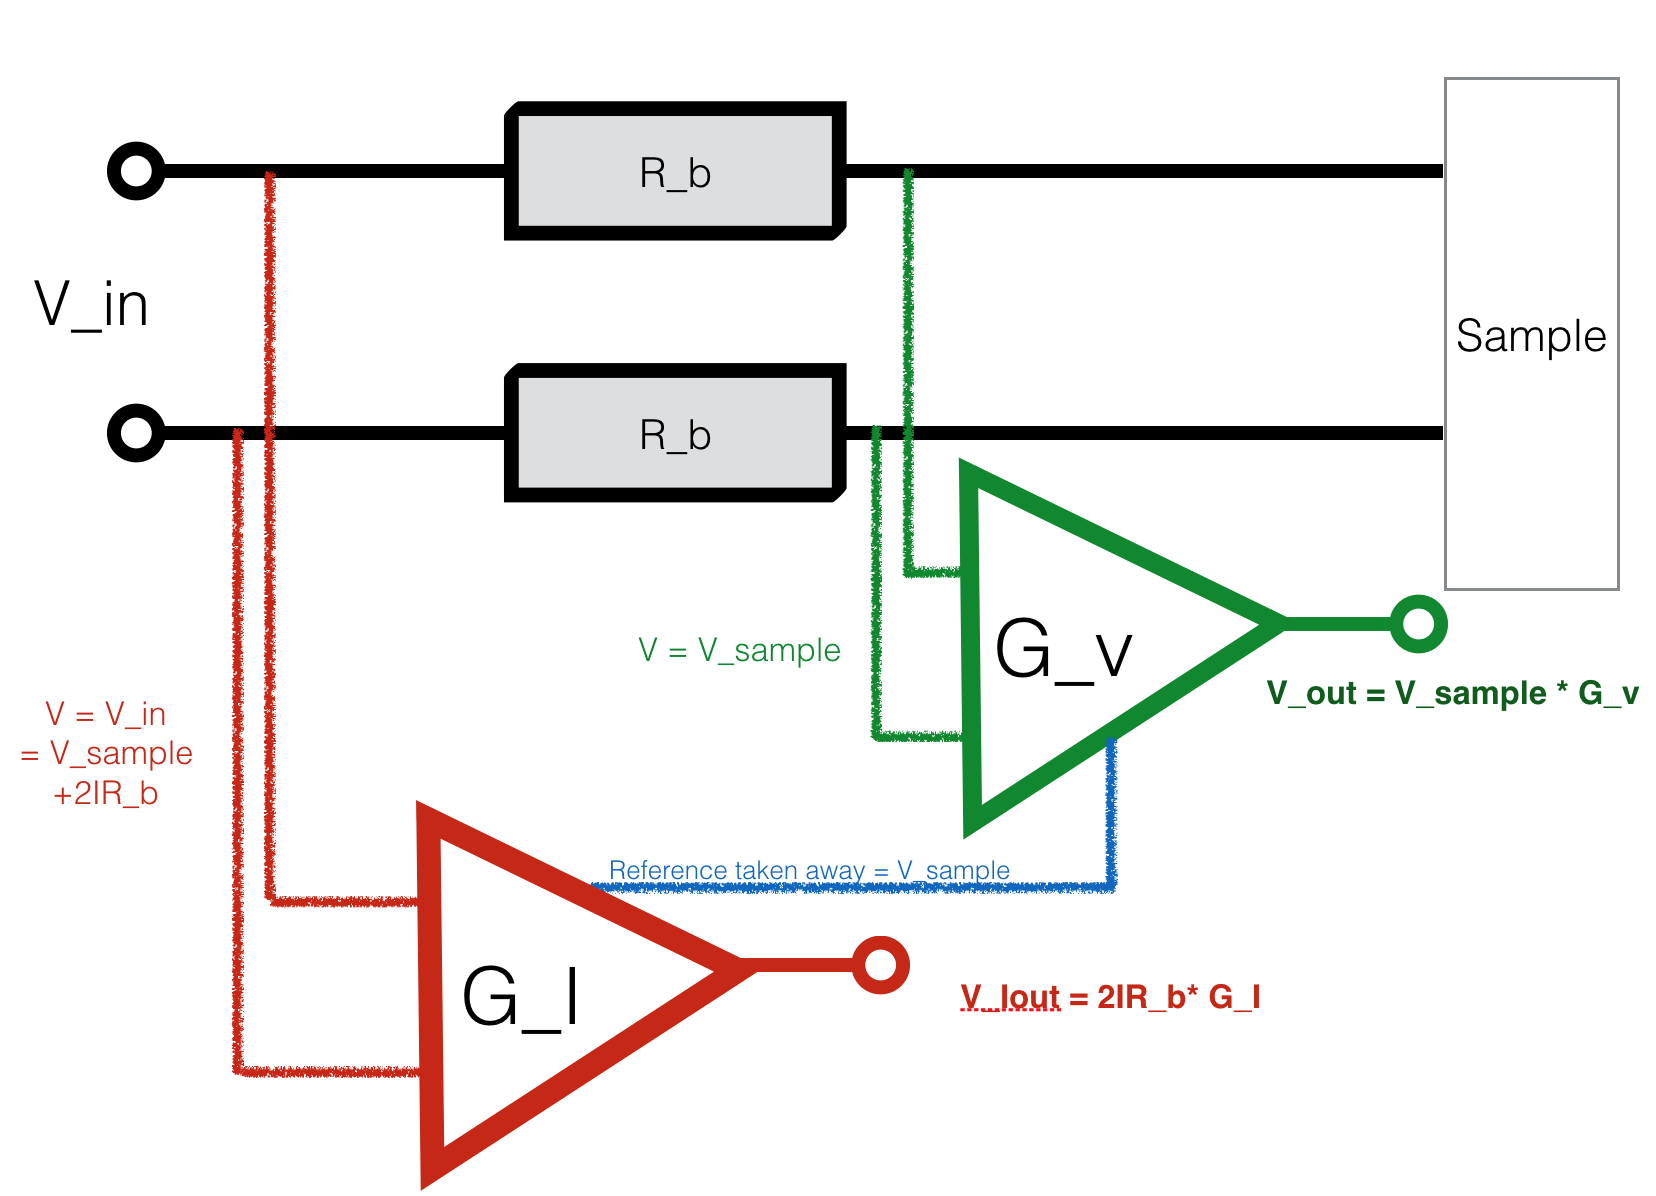
\includegraphics[height=9cm]{4terminal}
    \caption{Essentially   this  is   a  four   terminal  measurement
      configuration, where  the voltage  is measured  directly across
      the sample,  and the  current is  measured via  bias resistors,
      which all but nullify the internal resistances of the wires, to
      get a measurement going.}
    \label{fig:4t}
  \end{figure}

  The setup  is connected through  a box as  below. Pins are  used to
  connect laboratory wires with desired sample wires. There important
  rules are:


  \begin{figure}[h]
    \centering 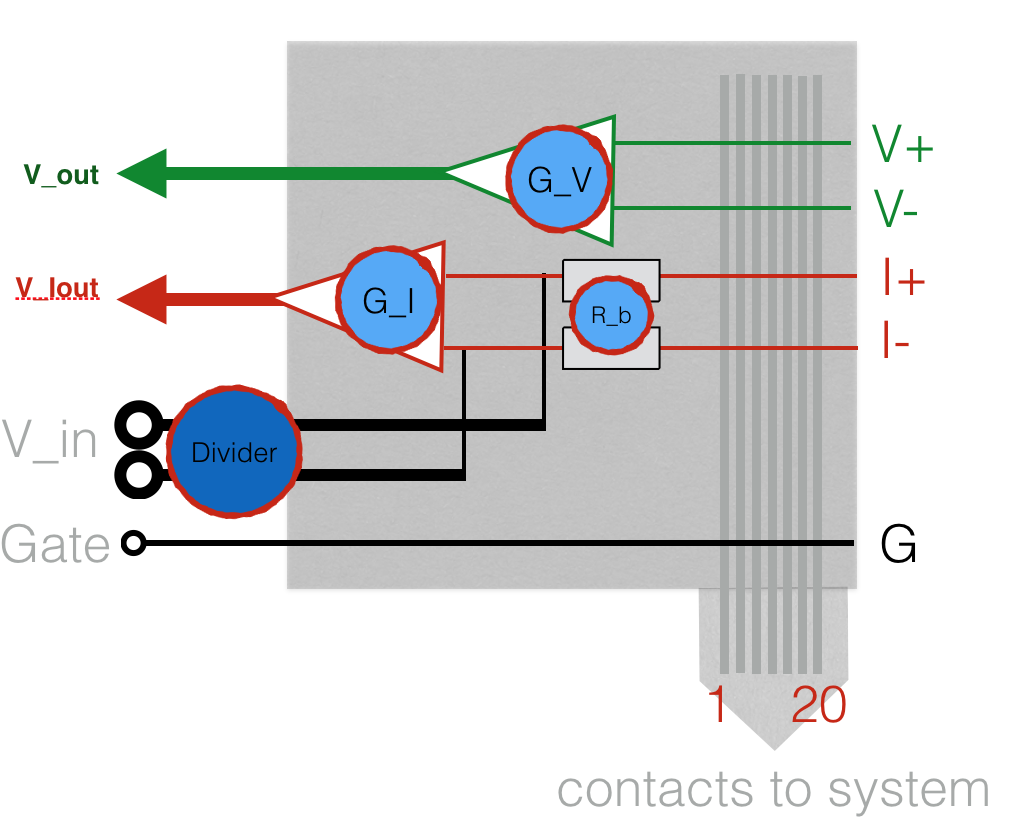
\includegraphics[height=9cm]{box}
    \caption{Dials  are  used to  choose  resistors  and gains.   The
      various  wires  to  the  sample   area  are  connected  to  the
      labortoary  wires   via  a   mesh,  that  connects   two  given
      cables. e.g. for a two terminal measurement, 2V+ 2I+ 3I- 3V- 5G
      (the coordinates of the pins that  we would place) and we would
      ground all remaining sample wires to a single ground. \red{VERY
        IMPORTANT TO GROUND V+ V- etc  when changing pins and put all
        sample wires common.}}
    \label{fig:box}
  \end{figure}
  \begin{itemize}
  \item  Pins at  6V+  connects V+  to the  6th  wire/contact on  the
    sample. Refer to a diagram to determine correct connection.
  \item  Whenever changing  connections,  ground  V+ V-  I+  I- G  by
    putting in pins at 12V+ 12V- 12I+ 12I- 12G where the 12th wire to
    the sample is in some way grounded;
  \item Whenever idle, to avoid potential difference build-up, ground
    all the sample wires as well e.g. put pins on 1G 2G 3G .. 20G, so
    that they are all grounded via the 12th sample wire;
  \end{itemize}

  \subsection{Connecting matrix}
  The  matrix allows  one  to  connect cables  in  the laboratory  to
  contacts on the samples. In  the image below: \textbf{Horizontal} -
  laboratory cables; \textbf{Vertical} - contacts to sample.


\begin{figure}[h]
  \centering
  \begin{minipage}{0.4\linewidth}
    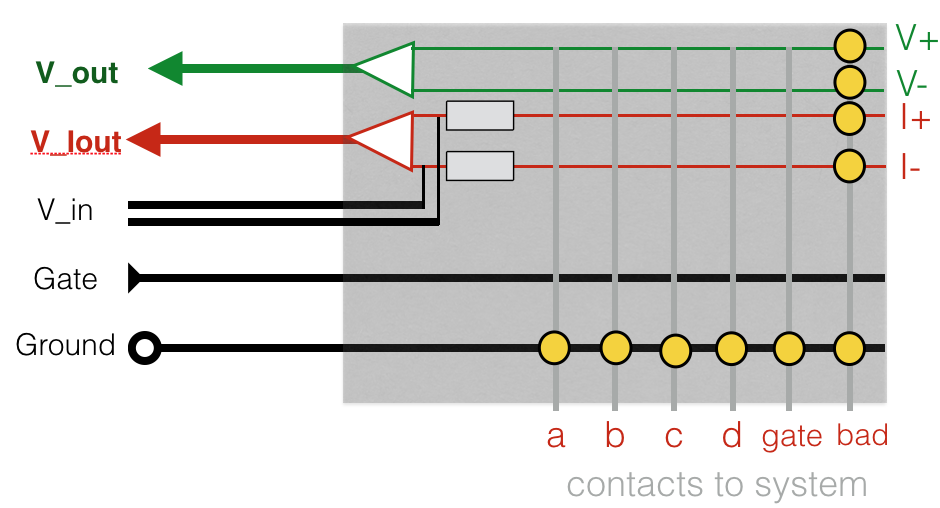
\includegraphics[width = \textwidth]{set1}
  \end{minipage}
  \begin{minipage}{0.4\linewidth}
    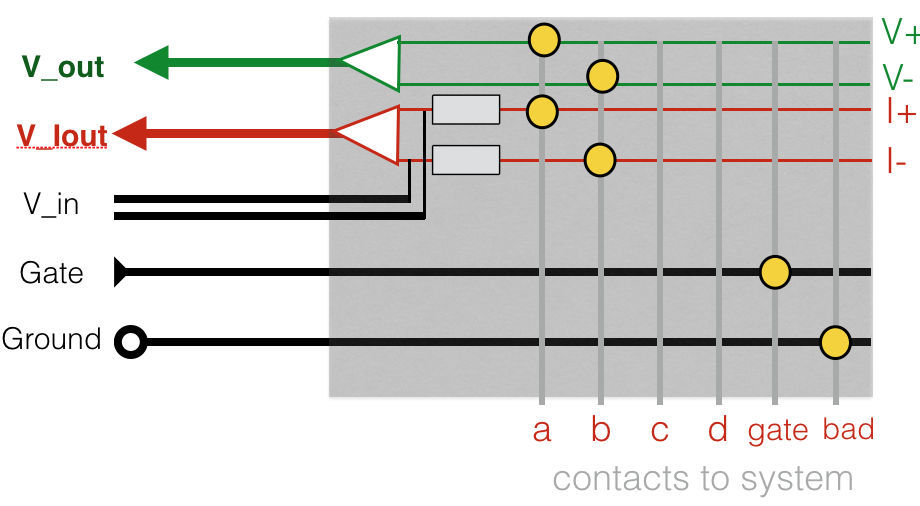
\includegraphics[width = \textwidth]{set2}
  \end{minipage}
  \begin{minipage}{0.4\linewidth}
    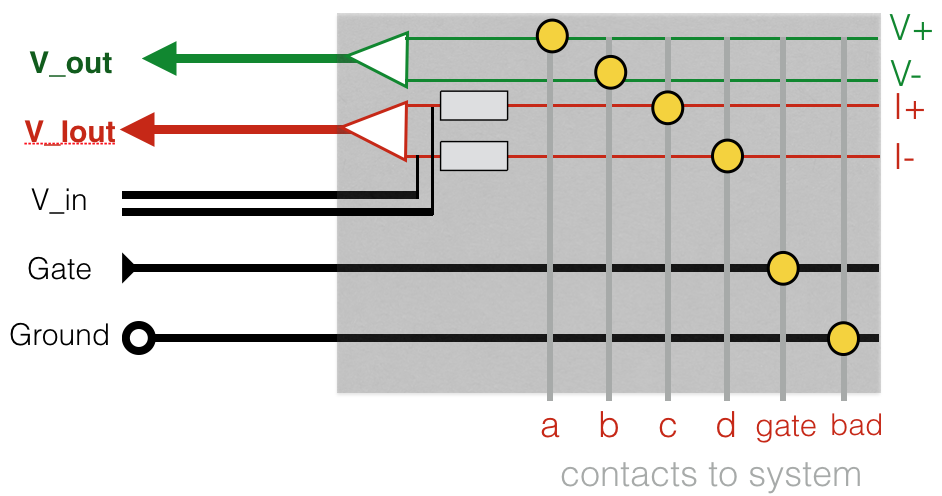
\includegraphics[width = \textwidth]{set3}
  \end{minipage}
\end{figure}
\begin{itemize}
\item \textbf{First  image shows} how  to ground all the  sample when
  not in use  and how to common ground the  laboratory cables via the
  bad contact.   \red{When putting new pins  in \ira put in  new pins
    \ira take  out the  four common  pins to  separate them  from the
    ground \ira take out ground pins.};
\item Configuration for two terminal measurement with gate;
\item Configuration for four terminal measurement with gate;
\end{itemize}

\subsection{Connection to Pre-Amp in the lab}
\begin{enumerate}
\item \cmd{Connect the power cable  from the \quote{blue box} +5V to
    the pre-amp};
\item  \cmd{To  $  V_\text{in}  $  connect  the  voltage  cable  from
    \quote{Signal Output 2 Out} on the Lock In};
\item \cmd{$ V_\text{iout} $ to PXIe-4462 AI0};
\item \cmd{$ V_\text{out} $ (has blue tags) to PXIe-4462 AI3};
\item \cmd{Combine  $ V^{+} $,  $ I^{+}  $ and $  V^{-} $, $  I^{-} $
    together  in  pairs  using  a   $  \pi  $-connector  for  2-point
    measurement, or keep separate for 4-point};
\item \cmd{Open \quote{ziControl} and  click \quote{on} to turn the
    lock  in output  on for  the second  channel (or  the one  we are
    using)};
\item \cmd{Load \quote{IV\_va\_VR\ira IV\_BlueForce}};
\end{enumerate}


\newpage
